\subsection{getDocumentsPrinceton}
Request Type: \textbf{POST}
\newline
Request Address: \textbf{/getdocumentsprinceton}
\newline

This endpoint takes in a JSON document containing a defined number of days to query documents by into the past. The returned data will also be a JSON document that contains all \textbf{unique} documents found in the database that were uploaded inside the window of the provided amount of days.

It should be noted that this endpoint specifically checks for the existence of the "globalid" field to include only documents created by Shweta's uploader script. This will exclude all documents uploaded by the Adapt uploader script as it does not insert the "globalid" field when uploading.

\subsubsection{Data Format}
\textbf{Required Data}:
\newline
\newline
This endpoint takes in a JSON document in the request body using the format found in Figure \ref{fig:getdocumentsprinceton1}. The "Integer" field should be replaced with the number of days being used to query back to.
\begin{figure}[H]
    \centering
    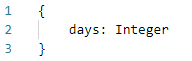
\includegraphics{img/getdocumentsprinceton1.PNG}
    \caption{getDocumentsPrinceton Received Data Format}
    \label{fig:getdocumentsprinceton1}
\end{figure}
\textbf{Returned Data}:
\newline
\newline
This endpoint will return a JSON document with a list that contains all unique MongoDB documents that were found within the amount of days provided in the POST request body. An example of what this JSON document looks like can be found in Figure \ref{fig:getdocumentsprinceton2}.

\begin{figure}[H]
    \centering
    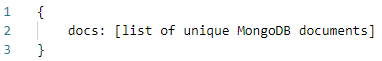
\includegraphics{img/getdocumentsprinceton2.PNG}
    \caption{getDocumentsPrinceton Returned Data Format}
    \label{fig:getdocumentsprinceton2}
\end{figure}
